\chapter{Visitor模式}
\section{访问者模式的概念}
\subsection{定义}
访问者(Visitor)模式的定义:将作用于某种数据结构中的各元素的操作分离出来封装成独立的类,使其在不改变数据结构的前提下可以添加作用于这些元素的新的操作,为数据结构中的每个元素提供多种访问方式。它将对数据的操作与数据结构进行分离,是行为类模式中最复杂的一种模式。
\subsection{优点}
访问者(Visitor)模式是一种对象行为型模式,优点如下:
\begin{enumerate}
	\item 扩展性好。能够在不修改对象结构中的元素的情况下,为对象结构中的元素添加新的功能。
	\item 复用性好。可以通过访问者来定义整个对象结构通用的功能,从而提高系统的复用程度。
	\item 灵活性好。访问者模式将数据结构与作用于结构上的操作解耦,使得操作集合可相对自由地演化而不影响系统的数据结构。
	\item 符合单一职责原则。访问者模式把相关的行为封装在一起,构成一个访问者,使每一个访问者的功能都比较单一。
\end{enumerate}
\subsection{缺点}
\begin{enumerate}
	\item 增加新的元素类很困难。在访问者模式中,每增加一个新的元素类,都要在每一个具体访问者类中增加相应的具体操作,这违背了“开闭原则”。
	\item 破坏封装。访问者模式中具体元素对访问者公布细节,这破坏了对象的封装性。
	\item 违反了依赖倒置原则。访问者模式依赖了具体类,而没有依赖抽象类。
\end{enumerate}
\subsection{模式的角色}
\begin{enumerate}
	\item Visitor访问者:定义一个访问具体元素的接口,为每个具体元素类对应一个访问操作 visit() ,该操作中的参数类型标识了被访问的具体元素。
	\item ConcreteVisitor具体访问者:实现抽象访问者角色中声明的各个访问操作,确定访问者访问一个元素时该做什么。
	\item Element元素:声明一个包含接受操作 accept() 的接口,被接受的访问者对象作为 accept() 方法的参数。
	\item ConcreteElement:实现抽象元素角色提供的 accept() 操作,其方法体通常都是 visitor.visit(this) ,另外具体元素中可能还包含本身业务逻辑的相关操作。
	\item ObjectStructure对象结构:是一个包含元素角色的容器,提供让访问者对象遍历容器中的所有元素的方法,通常由 List、Set、Map 等聚合类实现。
\end{enumerate}
\section{访问者模式实现——例一}
\begin{table}[!h]
	\begin{tabular}{|l|l|}
		\hline
		名字&说明\\
		\hline
		Visitor&表示访问者抽象类,它访问文件和文件夹\\
		\hline
		Element&表示数据结构的接口,接受访问者访问\\
		\hline
		ListVisitor&Visitor类的子类,显示文件和文件夹一览\\
		\hline
		Entry&File和Directory的父类,是抽象类,实现了Element接口\\
		\hline
		File&表示文件的类\\
		\hline
		Directory&表示文件夹的类\\
		\hline
		FileTreatementException&表示向文件中add时发生的异常类\\
		\hline
		Main&测试类\\
		\hline
	\end{tabular}
\end{table}
\begin{figure}[!h]
	\centering
	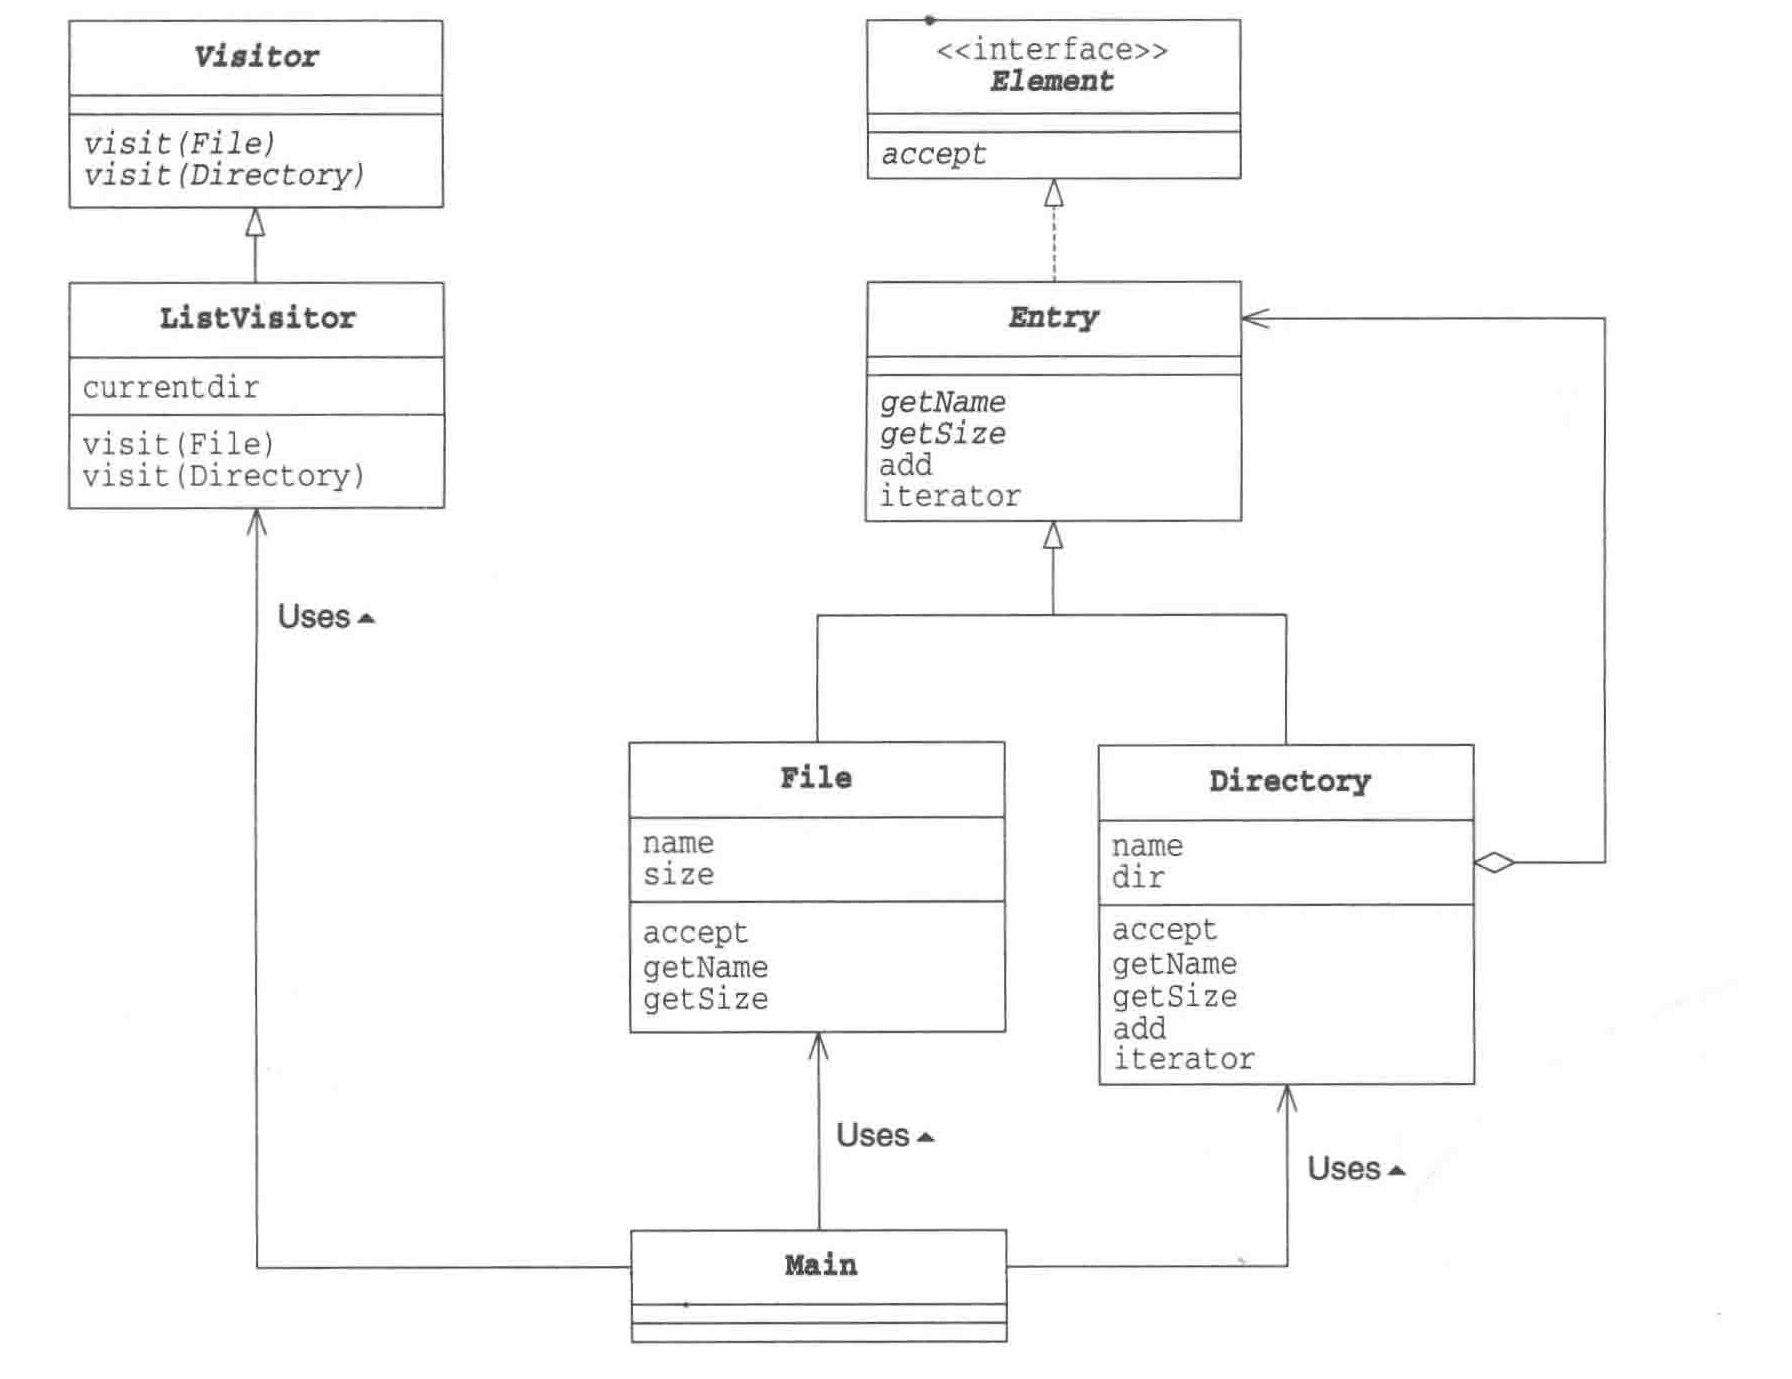
\includegraphics[width=\textwidth]{image/13-1}
	\caption{访问者模式类图}
\end{figure}
\begin{lstlisting}
public interface Element {
	void accept(Visitor visitor);
}
//防止对文件进行 add操作
public class FileTreatmentException extends RuntimeException {
	public FileTreatmentException() {}
	public FileTreatmentException(String msg) {
		super(msg);
	}
}
\end{lstlisting}
\begin{lstlisting}
//相当于 Composite 模式的父类,在 Visitor 模式中使用并不是必须的
//真正作为被访问者的是它的子类
public abstract class Entry implements Element {
public abstract String getName();
	public abstract int getSize();
	public Entry add(Entry entry) throws FileTreatmentException {
		throw new FileTreatmentException();
	}
	public String toString() {
		return getName() + " (" + getSize() + ")";
	}
}
\end{lstlisting}
\begin{lstlisting}
// 作为被访问的元素
public class File extends Entry {
	private String name;
	private int size;
	public File(String name, int size) {
		this.name = name;
		this.size = size;
	}
	public String getName() {
		return name;
	}
	public int getSize() {
		return size;
	}
	//告诉 Visitor 正在访问的对象是 File 的实例
	public void accept(Visitor visitor) {
		visitor.visit(this);
	}
}
\end{lstlisting}
\begin{lstlisting}
public class Directory extends Entry {
	private String name;
	private List<Entry> dir = new ArrayList<>();
	public Directory(String name) {
		this.name = name;
	}
	public String getName() {
		return name;
	}
	public int getSize() {
		int size = 0;
		Iterator<Entry> it = dir.iterator();
		while (it.hasNext()) {
			Entry entry = it.next();
			size += entry.getSize();
		}
		return size;
	}
	public Entry add(Entry entry) throws FileTreatmentException {
		dir.add(entry);
		return this;
	}
	public Iterator<Entry> iterator() {
		return dir.iterator();
	}
	public void accept(Visitor visitor) {
		visitor.visit(this);
	}
}
\end{lstlisting}
\begin{lstlisting}
//表示访问者的抽象类,依赖于访问的数据结构
public abstract class Visitor {
	//根据不同的参数调用不同的访问方法
	public abstract void visit(File file);
	public abstract void visit(Directory directory);
}
\end{lstlisting}
\begin{lstlisting}
public class ListVisitor extends Visitor {
	//当前访问的文件夹的名字
	private String currentDir = "";
	public void visit(File file) {
		System.out.println(currentDir + "/" + file);
	}
	public void visit(Directory directory) {
		System.out.println(currentDir + "/" + directory);
		String saveDir = currentDir;
		currentDir = currentDir + "/" + directory.getName();
		Iterator<Entry> it = directory.iterator();
		while (it.hasNext()) {
			Entry entry = it.next();
			entry.accept(this);
		}
		currentDir = saveDir;
	}
}
\end{lstlisting}
\begin{lstlisting}
public class Main {
	public static void main(String[] args) {
		try {
			System.out.println("Making root entries");
			Directory rootDir = new Directory("root");
			Directory binDir = new Directory("bin");
			Directory tmpDir = new Directory("tmp");
			Directory usrDir = new Directory("usr");
			rootDir.add(binDir);
			rootDir.add(tmpDir);
			rootDir.add(usrDir);
			binDir.add(new File("vi", 10000));
			binDir.add(new File("latex", 20000));
			rootDir.accept(new ListVisitor());
			
			System.out.println("");
			System.out.println("Making user entries");
			Directory yuki = new Directory("yuki");
			Directory hanako = new Directory("hanako");
			Directory tomura = new Directory("tomura");
			usrDir.add(yuki);
			usrDir.add(hanako);
			usrDir.add(tomura);
			yuki.add(new File("diary.html", 100));
			yuki.add(new File("Composite.java", 200));
			hanako.add(new File("memo.tex", 300));
			tomura.add(new File("game.doc", 400));
			tomura.add(new File("junk.mail", 500));
			rootDir.accept(new ListVisitor());
		} catch (FileTreatmentException e) {
			e.printStackTrace();
		}
	}
}
\end{lstlisting}
\section{访问者模式实现——例二}
\begin{figure}[!h]
	\centering
	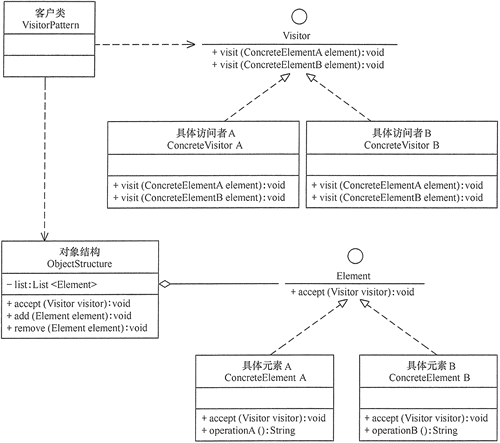
\includegraphics[width=0.8\textwidth]{image/13-2}
	\caption{text}
\end{figure}
\begin{lstlisting}
//抽象访问者
interface Visitor {
	void visit(ConcreteElementA element);
	void visit(ConcreteElementB element);
}

//具体访问者A类
class ConcreteVisitorA implements Visitor {
	public void visit(ConcreteElementA element) {
		System.out.println("具体访问者A访问-->" + element.operationA());
	}
	
	public void visit(ConcreteElementB element) {
		System.out.println("具体访问者A访问-->" + element.operationB());
	}
}

//具体访问者B类
class ConcreteVisitorB implements Visitor {
	public void visit(ConcreteElementA element) {
		System.out.println("具体访问者B访问-->" + element.operationA());
	}
	
	public void visit(ConcreteElementB element) {
		System.out.println("具体访问者B访问-->" + element.operationB());
	}
}
\end{lstlisting}
\begin{lstlisting}
//抽象元素类
interface Element {
	void accept(Visitor visitor);
}

//具体元素A类
class ConcreteElementA implements Element {
	public void accept(Visitor visitor) {
		visitor.visit(this);
	}
	
	public String operationA() {
		return "具体元素A的操作。";
	}
}

//具体元素B类
class ConcreteElementB implements Element {
	public void accept(Visitor visitor) {
		visitor.visit(this);
	}
	
	public String operationB() {
		return "具体元素B的操作。";
	}
}

//对象结构角色
class ObjectStructure {
	private List<Element> list = new ArrayList<Element>();
	
	public void accept(Visitor visitor) {
		Iterator<Element> i = list.iterator();
		while (i.hasNext()) {
			((Element) i.next()).accept(visitor);
		}
	}
	
	public void add(Element element) {
		list.add(element);
	}
	
	public void remove(Element element) {
		list.remove(element);
	}
}
\end{lstlisting}
\begin{lstlisting}
public class VisitorPattern {
	public static void main(String[] args) {
		ObjectStructure os = new ObjectStructure();
		os.add(new ConcreteElementA());
		os.add(new ConcreteElementB());
		Visitor visitor = new ConcreteVisitorA();
		os.accept(visitor);
		System.out.println("------------------------");
		visitor = new ConcreteVisitorB();
		os.accept(visitor);
	}
}
\end{lstlisting}
\begin{lstlisting}
//output
具体访问者A访问-->具体元素A的操作。
具体访问者A访问-->具体元素B的操作。
------------------------
具体访问者B访问-->具体元素A的操作。
具体访问者B访问-->具体元素B的操作。
\end{lstlisting}
\section{扩展思路}
\begin{enumerate}
	\item 双重分发:在Visitor模式中,ConcreteElement和ConcreteVisitor共同决定了实际进行的的处理。
	\item 为什么弄这么复杂?Visitor目的是将处理从数据结构中分离出来,提供了组件的独立性。
	\item 开闭原则:对扩展开放,对修改关闭;
	\item 易于增加ConcreteVisitor角色;
	\item 难以增加ConcreteElement角色,需要修改Visitor;
	\item Visitor实现了数据结构和处理的分离,访问者必须从数据结构中获取足够多信息才能工作。
\end{enumerate}
\section{相关设计模式}
\begin{enumerate}
	\item Iterator模式和Visitor都是在某种数据机构上处理,Iterator用于逐个遍历
	保存在数据结构中的元素;Visitor用于保存数据结构中的元素进行某种特定处理。
	\item 有时Visitor会使用Composite。
	\item Interpreter模式有时会使用Visitor。
\end{enumerate}